\documentclass[10pt]{article}
%\documentclass[10pt,twocolumn]{article}
\usepackage{fullpage}

% For revision control
%\usepackage{rcs-multi}
%\rcsid{$Id$}
%\rcsid{$Header$}
%\rcskwsave{$Author$}
%\rcskwsave{$Date$} 
%\rcskwsave{$Revision$}
%%\rcsRegisterAuthor{devangel}{Dennis Jos{\'e} Evangelista}
%\rcsRegisterAuthor{devangel}{Dennis J. Evangelista}

% I typically use these
\usepackage{graphicx}
\usepackage{color}
\usepackage{makeidx}
\usepackage{siunitx}

% PDF metadata
\usepackage{hyperref}
\hypersetup{pdftitle={Longitudinal plane aerodynamics of Southeast Asian flying lizards (Agamidae: Draco}}
\hypersetup{pdfauthor={D. Evangelista, J. McGuire and R. Dudley}}
\hypersetup{pdfsubject={biology}}
\hypersetup{pdfkeywords={biomechanics, evolution, Draco, physical model, aerodynamics, gliding, stability}}

% Biology style references
\usepackage[round]{natbib}
\setcitestyle{authoryear, round, comma, aysep={;}, yysep={,}, notesep={, }}
\bibliographystyle{apalike}

% Figures at end for draft
%\usepackage[lists,tablesfirst]{endfloat}

% Genus and species names
\newcommand{\Draco}{\emph{Draco}}
\newcommand{\Dracomelanopogon}{\emph{Draco melanopogon}}
\newcommand{\Dracomaximus}{\emph{Draco maximus}}
\newcommand{\Dmelanopogon}{\emph{D. melanopogon}}
\newcommand{\Dmaximus}{\emph{D. maximus}}
\newcommand{\by}{$\times$}


\title{Longitudinal plane aerodynamics of Southeast Asian flying lizards (Agamidae: \Draco)}
\author{D. Evangelista, J. McGuire and R. Dudley}
\date{\today}

\begin{document}
\maketitle
\begin{abstract}
This paper describes wind tunnel tests of models of \Draco\ lizards and computer simulations of their longitudinal plane dynamics during a glide.  Data already taken includes force and moment coefficients and baseline stability of a \Draco\ shape, as well as measurements of the effect of camber and of  completely flat body forms.  In addition, data was taken on hypothetical \Draco-like shapes with no patagia, half-patagia, and double-sized patagia.  Work that remains to be done includes the computer simulations and comparison to actual trajectories, computation of stability and glide metrics, and consideration of how these metrics change during a transition from no to half to a whole to a double sized wing. This paper fits with the rest of thesis work as a validation of using physical models in this way as well as questions of morphology changes and their effect on flight performance. I have not yet asked Robert where an appropriate home for this paper would be. 
\end{abstract}

\section{Introduction}
Still need to write this. 

\section{Methods and materials}
\subsection{Models and test conditions}
Full scale models of \Dracomaximus\ (mass X, snout-vent length X)were constructed from published drawings and photographs and examination of fluid-preserved \Draco\ specimens in the University of California Museum of Vertebrate Zoology \citep{McGuire:2003, McGuire:2005, Savile:1962, Hairston:1957}.  Models were built on an aluminum plate with polymer clay (Polyform Products Co., Elk Grove, IL) to fill out the body and polymer clay on steel wire to form limbs.  Ribs, made of steel wire, were bent to shape using photographs, and patagia were constructed over the ribs using paper and paper surgical tape (3M, St. Paul, Minnesota).

Two postures were created to examine longitudinal plane maneuvers: a relatively flat midglide model and a highly cambered model corresponding to postures observed in the initial part of the glide \citep{McGuire:2003}.  In addition, body forms not observed in extant \Draco\ lizards were created to examine the effect of changes in morphology.  A model with no wings was created using the \Draco\ body shape without an attached patagium.  Patagia with the ribs trimmed to half their length and with the ribs extended to twice their length were also built, in order to test the effects of a half-wing or a longer wing.  The longer wing corresponds to the reconstructed wing shape of FOSSIL GUY (cite).  To provide a comparison to a simple shape without the anatomical details of a \Draco\ patagium, a \num{0.118}-inch (\SI{3}{\milli\meter}) flat acrylic plate with the same planform as the other models was used.  

For angle-of-attack runs, at least five replicates were conducted at \ang{15} angle increments from \numrange{-15}{90} degrees angle-of-attack.  Most runs were conducted at \SI{7}{\meter\per\second}, corresponding to typical glide speeds of \Dracomaximus\ \citep{McGuire:2005}. Angle-of-attack runs were also conducted at \SI{3}{\meter\per\second}, corresponding to a typical glide Reynolds number for \Dracomelanopogon\ \citep{McGuire:2005}, and at \SI{12}{\meter\per\second} to examine speeds beyond those normally encountered by \Draco.  Some runs were also conducted with smaller angle-of-attack increments to further examine the shape of the curve.  In addition, to further examine the effect of Reynolds number, speed runs were also conducted at zero angle-of-attack and speeds between \SIrange{0}{12}{\meter\per\second}.   

\subsection{Force measurements and flow visualization}
Models were mounted on a six-axis force transducer (ATI Industrial Automation, Apex, NC), which was in turn mounted on a 1/2-inch (\SI{1.27}{\centi\meter}) aluminum rod held by a 1-inch (\SI{2.54}{\centi\meter}) arm bolted to the wall of the wind tunnel.  The rod exited the model dorsally and posteriorly, in order to keep the sting downstream of the model during angle-of-attack tests.  Wind tunnel tests were conducted in an open-circuit Eiffel-type wind tunnel with an \num{18 x 18 x 36}-inch (\SI{45.7 x 45.7 x 91.4}{\centi\meter}) working section (Engineering Laboratory Design, Lake City, MN).  

Force transducer readings were recorded at \SI{1000}{\hertz} sampling frequency using a National Instruments 6251 data acquisition card (National Instruments, Austin, TX).  Raw measurements were rotated from a frame fixed to the model to one aligned with the wind tunnel and flow using the angle-of-attack.  Transformed measurements were then averaged over a one-minute recording.  For each measurement, wind tunnel speed $v$ was recorded and used to compute Reynolds number ($\mbox{Re} = vL/\nu$, $\nu = \SI{1e-6}{\meter\squared\per\second}$).  Lift $L$, drag $D$, and pitching moment $M_p$ were normalized to obtain nondimensional lift, drag, and pitching moment coefficients according to the following: 
\begin{equation}
C_L = \frac{L}{1/2 \rho v^2 A_p}
\end{equation}
\begin{equation}
C_D = \frac{D}{1/2 \rho v^2 A_p}
\end{equation}
\begin{equation}
C_m = \frac{M_p}{1/2 \rho v^2 A_p \lambda_{SVL}}
\end{equation}
where $\rho=\SI{1.204}{\kilo\gram\per\meter\cubed}$ is the air density, $A_p$ is the model planform area, and $\lambda_{SVL}$ is the snout-vent length of the model. 

Particle imaging velocimetry (PIV), in which paired images of particles suspended in the flow are used to obtain two-dimensional flow fields, was used to visualize flow in the sagittal plane at approximately half of the span of the patagium.  The flow was seeded using an olive oil mist created by a pressurized oil container equipped with a perforated tube atomizer (LaVision, G\"ottingen, Germany). Models were illuminated in the sagittal plane using a vertical \SI{532}{\nano\meter} wavelength laser sheet generated by a double-pulsed Nd:YAG laser (New Wave Research model 25185, Fremont, CA) equipped with a \ang{20} sheet optic.  The sheet was filmed with a LaVision ImagerPro X 2M camera and a Nikon \SI{50}{\milli\meter} f/1.8 lens to obtain paired images at \SI{15}{pairs\per\second}.  To obtain velocity fields, images were post-processed in DaVis (LaVision, G\"ottingen, Germany) with multiple passes up to \num{64 x 64} pixel windows at 75\% overlap.

\subsection{Additional analysis}
Introduce Koehl metrics here. Statistical analyses were performed in R \citep{R:2009}.

\subsection{Simulations}
Simulations will be conducted in Python.  Fill in the details here. 

\section{Results}
Fig.~\ref{fig:lift_aoa} shows the lift, drag, and pitching moment coefficients for the flat midglide and cambered initial glide models as functions of angle of attack.  I still need to add the cartoons and notes to the various figures that I have on the pencil version of this paper. 

\begin{figure}
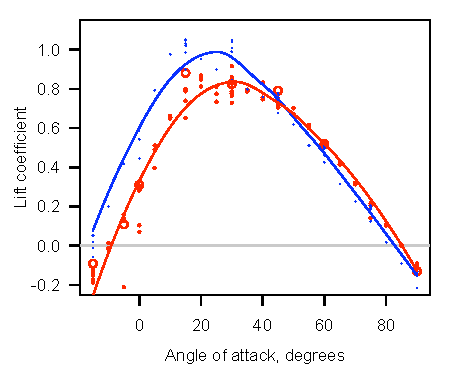
\includegraphics{figures/lift_v_aoa.pdf} 
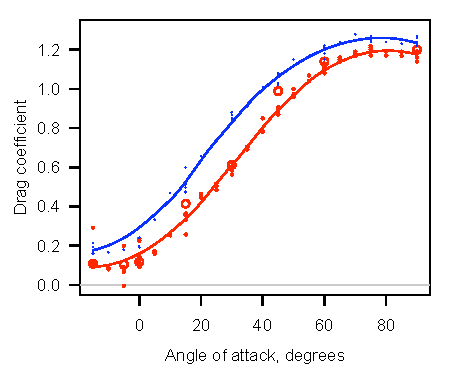
\includegraphics{figures/drag_v_aoa.pdf} 
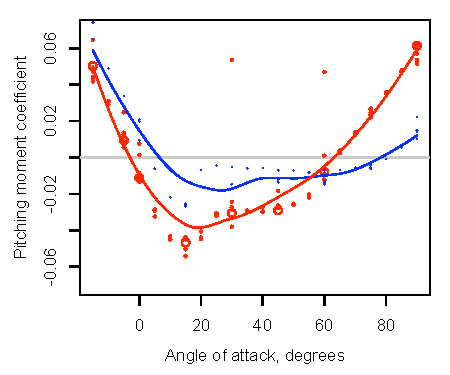
\includegraphics{figures/pitch_v_aoa.pdf} 
\caption{$C_L$, $C_D$, and $C_M$ versus angle of attack.  Flat midglide posture shown in red; cambered initial glide position shown in blue.  Open circles indicate tests at \Dmelanopogon\ Reynolds number; all other tests were completed at \Dmaximus\ Reynolds number.  Lines indicate locally weighted scatter plot loess smoothing.}
\label{fig:lift_aoa}
\end{figure}

\begin{figure}
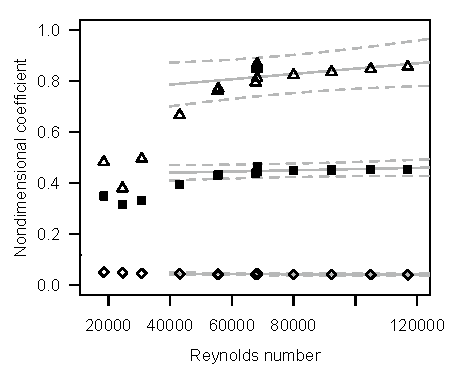
\includegraphics{figures/coeffs_v_Re.pdf}
\caption{Dependence of $C_L$ (open triangles), $C_D$ (filled squares), and $C_M$ (open diamonds) on Reynolds number.  Over the range of Reynolds numbers experienced by \Draco\ lizards, about 50,000 to 70,000, slopes are not significantly different from zero (linear regression, $p=0.06483$ for $C_L$, $p=0.2077$ for $C_D$, $p=0.1555$ for $C_M$).}
\label{fig:coeffs_Re}
\end{figure}

\begin{figure}
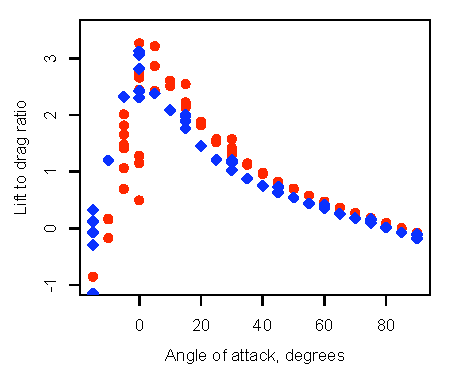
\includegraphics{figures/LD_v_aoa.pdf}
\caption{Lift to drag ratio versus angle of attack for flat midglide (red) and cambered initial glide (blue) postures.  The 95\% quantile lift-to-drag ratio is 2.7 for the flat posture and 2.5 for the cambered posture, corresponding to glide angles of 20.3 and 21.8 degrees respectively.  The absolute maximum lift-to-drag ratios are 3.2 and 3.1 for flat and cambered postures, corresponding to glide angles of \ang{17.0} and \ang{17.7}.}
\label{fig:LD_v_aoa}
\end{figure}

\begin{figure}
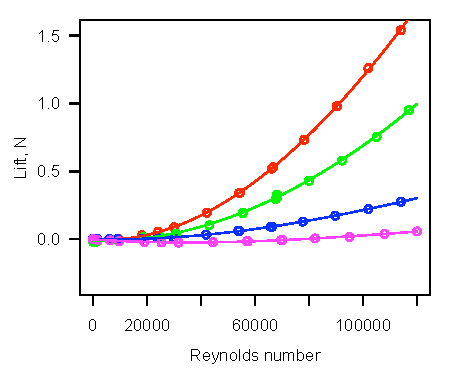
\includegraphics{figures/L_v_Re.pdf}
\caption{Lift versus Reynolds number for no wings, half wings, \Draco, and double wings.  Need to add dot indicating \Dmelanopogon\ and \Dmaximus\ operating points and weights to indicate force production margin.  Some of the effect here is due to area. }
\label{fig:L_v_Re}
\end{figure}

\begin{figure}
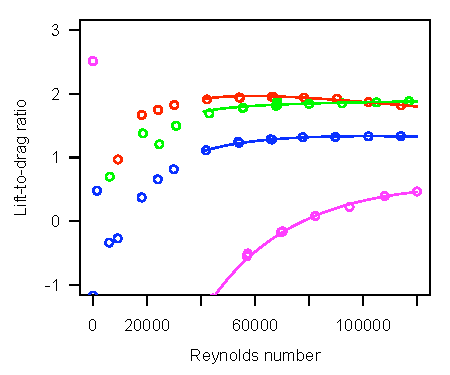
\includegraphics{figures/LD_v_Re.pdf}
\caption{Lift-to-drag ratio versus Reynolds number for no wings, half wings, \Draco, and double wings.  Area effects are normalized out here so that all we see is the effect of wing aspect ratio.  There is slight improvement as wing aspect ratio is increased.  Need to add cartoons.}
\label{fig:LD_v_Re}
\end{figure}

\begin{figure}
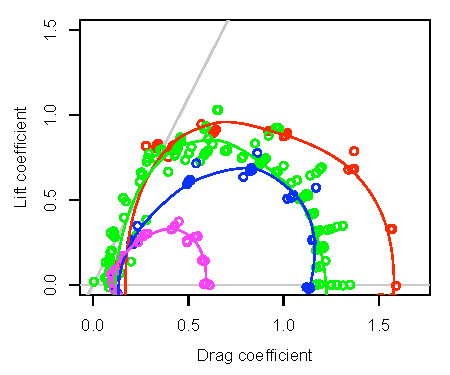
\includegraphics{figures/Cl_v_Cd_wings.pdf}
\caption{Lift coefficient versus drag coefficient for no wings, half wings, \Draco, and double wings.  Going from no wings to half wings vastly improves the parachuting performance.  Further increases in wing do not greatly alter parachuting performance, but do improve glide angle. }
\label{fig:Cl_v_Cd_wings}
\end{figure}

\begin{figure}
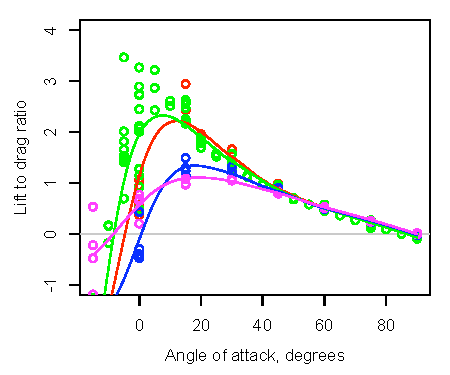
\includegraphics{figures/LD_v_aoa_wings.pdf}
\caption{Lift-to-drag ratio versus angle of attack for no wings, half wings, \Draco, and double wings.  This plot confirms that further incrases in wing improve glide angle.}
\label{fig:LD_v_aoa_wings}
\end{figure}

\begin{figure}
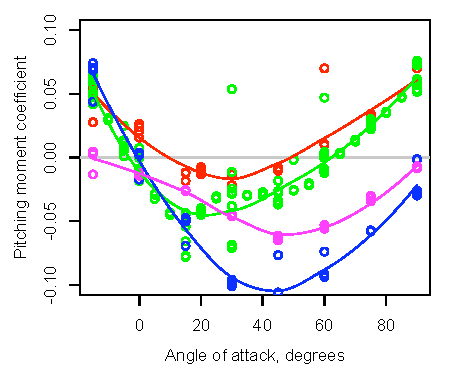
\includegraphics{figures/Cm_v_aoa_wings.pdf}
\caption{Pitching moment coefficient versus angle of attack for no wings, half wings, \Draco, and double wings.  A double wing may have a large area and might be expected to be a great parachute... but it is not stable?  Need to add tail on this plot.}
\label{fig:Cm_v_aoa_wings}
\end{figure}

\section{Discussion}

\subsection{\Draco\ aerodynamics}
\Draco\ flies in a regime where force coefficients are independent of Reynolds number. The aerodynamic force coefficients experienced by the smallest \Draco\ lizards are similar to those experienced by the largest. The measurements suggest an animal half the size of \Dmelanopogon\ would experience a drop in lift coefficient; it would be interesting to check the minimum size that \Draco\ young start to effectively glide or the ancestral size predicted from phylogenetic ancestral state reconstruction. 

The cambered posture taken during the initial glide increases the lift coefficient.  This would improve the ability to generate forces at low speed during the initial part of the glide.  The flat midglide posture is slightly more stable and has a lower drag coefficients; this would improve flight ability at higher speeds.  

Lift to drag ratios correspond to glide angles of at best \ang{17}, \ang{20} (95th percentile).  These are steeper angles than \Draco\ does?  This would suggest (1) steeper glide angles during the initial glide to improve maneuverability during take off and during a dangerous low speed phase; (2) faster, flatter, midglide trajectories and deceleration especially near the end of the glide, to soften landings.  In other words, perhaps equilibrium glide angles are not super predictive of the actual instantaneous behavior, they only reflect the overall... 

Do simulations to back this up. 

\subsection{What is the use of half a wing?}
Adding wings improves gliding performance by increasing the area and by modestly improving lift coefficients. 

People normally focus on L/D ratio.  Early in addition of wings, the largest performance gains may be in alternative metrics of performance like parachuting performance (Fig 6).  Further additions to the wings make improvements in gliding peformance (Fig. 7).  The ability to exploit such performance improvements is constrained by stability (Fig 8 and the new Yonatan plot).  

\subsection{How do stability and glide metrics change as morphology is changed}

\subsection{Place these on a phylogeny? and consider convergent versions of Draco in fossil record}

\section*{Acknowledgements}
We thank the students of UC Berkeley's spring 2009 Mechanics of Organisms (IB135L) class for collection of some of the force measurements and all of the flow visualization.  We also thank Felicia Linn, Louise Qu, Yonatan Munk, Aaron Hoover, Kevin Peterson and the Koehl and Fearing Labs at UC Berkeley for assistance in construction of models, and Tom Libby and the Berkeley Center for Integrative Biomechanics in Education and Research (CIBER) for use of the force sensor.
\bibliography{references/draco}
\end{document}